\documentclass{beamer}
  \usetheme{metropolis}
  \setbeamercovered{invisible}
  \setbeamertemplate{navigation symbols}{}
  \setbeamertemplate{footline}{\hfill\insertframenumber\hfill\vspace{3mm}}
  \usetikzlibrary{matrix}
  
  \usepackage[normalem]{ulem}
  \usepackage{stmaryrd}
  % \usepackage{minted}
  \usepackage{tikz}
  \usepackage{tikz-cd}
  \let\OLDitemize\itemize
  \renewcommand\itemize{\OLDitemize\addtolength{\itemsep}{150pt}}
  \newcommand{\Turnsi}[2]
	{ {#1}\vdash  {#2}}

  \usepackage{outlines}
  
         % Use metropolis theme
         \usepackage{mathpartir}
         \usepackage{mathtools}
         \usepackage{appendixnumberbeamer}
         
         \usepackage{booktabs}
         \usepackage[scale=2]{ccicons}
         
         \usepackage{pgfplots}
         \usepgfplotslibrary{dateplot}
         
         \usepackage{xspace}
         \newcommand{\themename}{\textbf{\textsc{metropolis}}\xspace}
  \title{A reading of justification logic modality in Curry-Howard fashion}
  \date{\today}
  \author{Konstantinos Pouliasis}
  \institute{CUNY, Graduate Center}
  \begin{document}
    \maketitle
    \section{Introduction}
    \begin{frame}{Curry--Howard Isomorphism}
      \begin{itemize}
\item[] Sparked from the investigation of the connection of 
explicit proofs in intuitionistic logic and 
programs of a simple programming language (\emph{Simply Typed Lamda Calculus})

\item[] Central topic of study in the field of type theory

\item[] Standard theoretical tool for studying and designing programming languages
      \end{itemize}
\end{frame}
\begin{frame}{\emph{CHI} and logic}
  \begin{itemize}

  \item[] A  paradigm that emphasizes proof relevance
  \item[] The view of propositions--as--types has been extended to many logics
  \item[] As a result it can capture more complex programming language features. 
   (\textbf{scalability})
  \end{itemize}
\end{frame}
\begin{frame}{Justification logic}
  \begin{itemize}
    \item[] A logic of (explicitly) witnessed modality
    \item[] Started as a solution to the problem  of providing 
    constructive semantics to intuitionistic logic via explicit provability
    \item [] A proof relevant analysis of $S4$ modality 
    \item[] Scales to other systems of modal logic
    \item[] Applications in epistemology, epistemic game theory and programming language theory
  \end{itemize}
\end{frame}

\section{Intuitionistic Logic and STLC} 
\begin{frame}{Intuitionism and constructive mathematics}
  \begin{outline}
    \1[] {Continuation of Brouwer's program}
    
    \2[!]{Notion of truth collides with the notion of proof}
    
  \1[] Mathematical reasoning and logic is a human faculty
  
  \2[!] The creative subjects use mathematical language 
  as a means to express their reasoning (proof) constructs
  \2[!] 
  There are open problems
  \2[!] 
  Propositions do not come with a pre-existing truth value
  \3[!!] 
  Default absence of excluded middle
  \2[!] As Heraclitus puts it truth is "an homodoxy (common belief) that each can individually witness"
\end{outline}
\end{frame}

\begin{frame}{Logic within constructive mathematics}
\begin{outline} 

\1[] The object of logic is the study of ``sane'' proof constructs 

\1[] The traditional chasm between ``syntax'' and ``semantics'' is no longer  very fruitful at least when “engineering” new logics.
\end{outline}
\begin{columns}[T,onlytextwidth]
  \column{0.5\textwidth}

    \begin{alertblock}{Verificationist}
    \begin{quote}The meaning of a connective is the ways that one can prove it\end{quote}
    \end{alertblock}


  \column{0.5\textwidth}

  \begin{exampleblock}{Pragmatist}
  \begin{quote} The meaning of a connective is the way one can use its proofs\end{quote}
  \end{exampleblock}
\end{columns}
\end{frame}
\begin{frame}{Example: rules $\wedge$}
  \begin{mathpar}
 \inferrule*[right=Intro] { {\begin{array}{c} \mathcal{D} \\ {A} \end{array} } \\{\begin{array}{c} \mathcal{E} \\ {B} \end{array} }} {A\wedge B} 
  \end{mathpar}
\[ \begin{array}{c c} \inferrule*[right=Elim1] { {\begin{array}{c} \\ \mathcal{D} \\ {A\wedge B} \end{array} }} {A} & \inferrule*[right=Elim2] { {\begin{array}{c} \\ \mathcal{D} \\ {A\wedge B} \end{array} }} {B} \end{array} \]
\end{frame}

\begin{frame}{Proof equality and harmony}
  \begin{itemize}
  \item[] Proof trees are objects of logic and - as mathematical objects - are equipped with equality

  \item[]\alert{Logic is “algebraized”}
  
  \item[]Equalities should provide for the ''harmony'' of the Introduction and Elimination rules 
  (constructors– destructors)
  
 \end{itemize}
\end{frame}
\begin{frame}{Harmony}
\begin{alertblock}{Elim rules are not too strong a.k.a Local Soundness}\end{alertblock}
    
      \[ \begin{array}{l c r} {\inferrule*[right=Elim1]{\inferrule*[right=Intro] { {\begin{array}{c} \mathcal{D}\\ {A} \end{array} } \\{\begin{array}{c} \mathcal{E} \\ {B} \end{array} }} {A\wedge B}}{A}} & = & {\begin{array}{c} \mathcal{D}\\ {A} \end{array} } \end{array} \]
      \[ \begin{array}{l c r} {\inferrule*[right=Elim2]{\inferrule*[right=Intro] { {\begin{array}{c} \mathcal{D}\\ {A} \end{array} } \\{\begin{array}{c} \mathcal{E} \\ {B} \end{array} }} {A\wedge B}}{B}} & = & {\begin{array}{c} \mathcal{E}\\ {B} \end{array} } \end{array} \]
\end{frame}
\begin{frame}{Harmony}
  \begin{columns}[T,onlytextwidth]
    \column{0.7\textwidth}
        \begin{exampleblock}{Elim rules are not too weak a.k.a Local completeness}
        \[\begin{array}{l c r} {\begin{array}{c} \mathcal{D}\\ {A\wedge B} \end{array} } 
        & = & {\inferrule*[right=Intro]{
          {\inferrule*[right=Elim1] { {
          \begin{array}{c} \mathcal{D}\\ {A\wedge B} \end{array} 
        } } {A}}\\ {\inferrule*[right=Elim2] { {\begin{array}{c} \mathcal{D}\\ {A\wedge B} \end{array} } } {B}}}
        {A\wedge B}
      } \end{array} \]
        \end{exampleblock}
  \end{columns}
\end{frame}
\begin{frame}{Example:  $\supset$ rules}
  \begin{mathpar}
  \inferrule*[Right=$\supset^{x}$]{{\begin{array}[b]{c} \overline{x:A}\\ {\mathcal{D}} \\ A   \end{array}} }{A\supset B }
  \and
  \inferrule*[]{{\begin{array}[b]{c} {\mathcal{D}} \\ A\supset B  \end{array}}\\ {\begin{array}[b]{c} {\mathcal{E}} \\ A  \end{array}}}{B}
    
  \end{mathpar}
\end{frame}
\begin{frame}{Harmony}
  \begin{columns}[T,onlytextwidth]
    \column{0.5\textwidth}
  \begin{alertblock}{Not too strong}\end{alertblock}    
   \[\begin{array}{c c c}
    {\inferrule{
    {\inferrule[]{
      {\begin{array}[b]{c} \overline{x:A}\\ {\mathcal{D}} \\ B  \end{array}}}{A \supset B }}\\
  {\begin{array}{c}\mathcal{E}\\{A }\end{array}}
  }
  { B }} & = &
    
        {\begin{array}[b]{c} \mathcal{E} \\ A  \\ {\mathcal{D}} \\ B  \end{array}} 
  
  \end{array}\]
  \column{0.5\textwidth}
\begin{exampleblock}{ Not too weak}\end{exampleblock}
  \[\begin{array}{c c c}
	{\begin{array}[b]{c}  {\mathcal{D}} \\ A\supset B  \end{array}}
			& = &
		
			{\inferrule{
				{\inferrule[]{
						{\begin{array}[b]{c}  {\mathcal{D}} \\ A\supset B  \end{array}}
							\\{\overline{x:A}}} 
							{ B }}}
				{A \supset B}
		}
	\end{array}\]
\end{columns}
\end{frame}
\begin{frame}{Calculi for free}
    \begin{itemize} 
      \item[] trees of $A$ with open $\Gamma$ $\mapsto$ {terms} ($\Gamma\vdash M:A$) (inhabitation judgments)
      \item[] local soundness $\mapsto$ $\beta$ reduction (equality judgments), 
      \item [] local completeness $\mapsto$ $\eta$ expansion (equality judgments)
      \end{itemize}
\end{frame}

\begin{frame}
\begin{mathpar}
  \inferrule*[right=Refl] {x:A\in\Gamma}{\Turnsi {\Gamma} { x:A }}
  
    \inferrule*[right=$\top$I] { } {\Turnsi {\Gamma} { \langle \rangle:\top }}
\end{mathpar}  
\begin{mathpar}
    \inferrule*[right=Tup] {\Turnsi {\Gamma} {M:A}\\{\Turnsi {\Gamma} { M^{'}:B}}} {\Turnsi {\Gamma} {  
      \langle M,M^{'}\rangle:A\times B }}
\end{mathpar}
\begin{mathpar}
      \inferrule*[right=LPrj] {\Turnsi {\Gamma} {M:A\times B }} {\Turnsi {\Gamma} {\operatorname{fst}(M):  A}}
      \and
      \inferrule*[right=RPrj] {\Turnsi {\Gamma} {M:A\times B}} {\Turnsi {\Gamma} {\operatorname{snd}(M):  B}}
\end{mathpar}
\begin{mathpar}
  \inferrule*[right=$\lambda-$Abs] {\Turnsi {\Gamma, x:A } 
  {M:B }} {\Turnsi {\Gamma} { \lambda x:A.\  M:A\rightarrow B }}
  \and
  \inferrule*[right=App] {\Turnsi {\Gamma} {M:A\rightarrow B }\\{\Turnsi {\Gamma} {M^{'}:A}}} {\Turnsi {\Gamma} {  (M M^{'}):B }}
\end{mathpar}

\end{frame}
\begin{frame}
  \alert{Plus equality judgments}
  e.g. \[\inferrule*[right=$\beta\supset$] 
  {{\Gamma,x:A\vdash M:B}\\ {\Gamma\vdash N:A}}
  {\Gamma\vdash(\lambda x:\phi.M)(N)=_{\beta} [N/x]M:B}\]
  \[\inferrule*[right=$\eta\supset$] 
  {{\Gamma\vdash f:A\supset B}}
  {\Gamma\vdash f =_{\eta}\lambda x:A.\ (f x):B}\]
  \alert{plus congruence axiomatization}
\end{frame}
\begin{frame}{Metatheory for (almost) free}
  \begin{outline}
    \1 []  The good old  way
        \2[!] Forget about variables/ terms/ equalities and prove that $\Gamma\vdash A$ 
        has an order theoretic model ($\Gamma^*\le\phi^* $ )

    \1[] Cut elimination (core of CHI)
      \2[!]  Create  restricted versions of your calculus/ proof trees:
      \3[!!] do not permit Elim - After- Intro/ $\beta$ redexes 
      \2[!] Prove that your restricted system of proof trees proves the same stuff 
      by inventing a corresponding sequent calculus and proving cut elimination
      \3[!!] consistency (no normal form for bottom)
      \2[!!] equality means equi-normalizibility (together with Church Rosser)

    \end{outline}
\end{frame}
% \begin{frame}
%   \begin{outline}
%   \1[] \textbf{In proof terms}\\
%   For any term $\Gamma\vdash M:A$ the process 
%   of fully $\eta$ expanding and then, $\beta$ reducing it ($M\rightarrow^{*}_\eta N\rightarrow_\beta^{*} O$) 
%   is terminating in a normal form
%   \2[!] Your programming language has an \textit{evaluation strategy}
%   \2[!] As a lemma you can show that the system cannot inhabit the $\bot$
%   with a closed term
%   \1[] Trivially, any two terms that map to the same normal form are provenly equal
%   in the system        
% \1[] Proving additionally Church Rosser you get:
%   \2[!] Any two terms that are equated in the system lead to the \textit{same} normal form
%   \end{outline}
% \end{frame}

\section{JCalc: Motivation}

\begin{frame}{Motivation}
  \[\inferrule*[right=\sout{Nec}] 
  {\vdash A} {\vdash \Box A}\]
  \[\inferrule*[right=$\Box_I$] 
  {{\vdash A}\\ {\vdash  {\sf J A}}} {\vdash \Box A}\]
\begin{outline}
  \1[] In JL the motivation is that ${\vdash A}$ is ${\sf Int}$ and
${\sf J A}$ is in ${\sf CL}$  so $J$ can be seen as an embedding.
\1[] In general the (justified) connective can be treated independently of the details
of the two deductive systems
\1[] \alert{"Necessitation stems from internalization/ validation"}
\end{outline}
\end{frame}
\begin{frame}{Deductive systems}  
  \begin{outline}
    A deductive system is a $\Gamma\vdash\phi$ relation with the following (minimal) properties:
    
  \1[] Reflexivity :
  
  \2[*]$A \in \Gamma \Longrightarrow \Gamma\vdash_{I}A$\\
  %$\phi \in \Delta \Longrightarrow \Delta\vdash_{J}\phi$
  \1[] Compositionality:
  
  \2[*]$\Gamma\vdash A$ and $\Gamma^{\prime}, A\vdash B \Longrightarrow \Gamma,\Gamma^{'}\vdash B$
  \1[] Top element:
  
  \2[*]$\Gamma\vdash\top $
  \end{outline}
\end{frame}

\begin{frame}{ Completeness in deductive systems}
  
  \begin{outline}
  \1[] A deductive system $J$ is complete for $I$ (or a conservative extension) iff  there exists mapping 
  $\llbracket \bullet \rrbracket: U_I\rightarrow U_J$ on propositions of $I$ into propositions of $J$
   s.t. 
   \2[*]$\Gamma\vdash_I A \Longrightarrow \llbracket\Gamma\rrbracket\vdash_J \llbracket A\rrbracket $
  \2[*] $\llbracket\top_I \rrbracket = \top_J$
  
  \2[*] For $\Gamma$ of the form $A_1,\ldots, A_n$: 
  \3[]$\llbracket\Gamma \rrbracket=\llbracket A_1 \rrbracket,\ldots, \llbracket A_n\rrbracket$
  \end{outline}
\end{frame}


\begin{frame}{ $\Box$ as double theoremhood}
  
  \begin{outline}
  \1[] When $J$ is complete with respect to $I$ then double theoremhood 
   $\langle \vdash A, \vdash \llbracket A \rrbracket\rangle$ 
  is a basic modality
  \1[!] Intuitively $A\vdash  B$ implies $\llbracket A\rrbracket \vdash \llbracket B\rrbracket$ 
    and thus a double proof of $A$ ($\Box A$)  gives a double proof of $B$($\Box B$) 
  \1[!] The basic rule of $K$ modality is admissible 
    $$\inferrule*[] {A\vdash B} {\Box A\vdash \Box B} $$  
  % \2[*] $\llbracket\top_I \rrbracket = \top_J$
  
  % \2[*] For $\Gamma$ of the form $A_1,\ldots, A_n$: 
  % %\3[]$\llbracket\Gamma \rrbracket=\llbracket A_1 \rrbracket,\ldots, \llbracket A_n\rrbracket$
  \end{outline}
\end{frame}


\begin{frame}{My thesis in a slide}
  \begin{outline}
    \1[!] A natural deduction  with three kinds of judgments: 
    \2[!] $\Gamma\vdash\sf {A}$  that follows intuitionistic logic 
    \2[!] $\llbracket\Gamma \rrbracket\vdash \llbracket A\rrbracket $ that axiomatizes
    the notion of conservative extension
    \2[!] $\Box \Gamma \vdash \Box A$ for "double theoremhood"
   \1[!] Its order theoretic semantics
   \1[!] Analysis  of the new connective a la Gentzen to get
   \2 [*]proof terms/trees and equalities/ reductions 
   \1[!] Its Cut elimination/ normalization
   \1[!] An implementation in the metatheoretic framework "Makam" (work in progress)
   \1[!] Some good reasons to think that this idea is extensible
\end{outline}
\end{frame}






\section{Jcalc: provability (the good old way)}
\begin{frame}{Type Universe}
  \begin{mathpar}
    \inferrule*[right= Atom] { } {P_k \in {\sf Prop_0}}
    \and
    \inferrule*[right=Top] { } {\top \in {\sf Prop_0}}
    \and
    \inferrule*[right=Conj] {{ A \in {\sf Prop_i }}\\ { B \in {\sf Prop_i}}} {  A \wedge B \in {\sf Prop_i} } 
    %\inferrule*[right=Bot] { } {\bot \in {\sf Prop_0}} 
    %\and
    \and
    \inferrule*[right=Box] { A \in{\sf Prop_{0} }} {\Box  A\in{\sf Prop_{1}} }
    %\and
    %\inferrule*[right= Arr] {{ A \in {\sf Prop_{i} }}\\ { B \in {\sf Prop_{j}}}} { A\supset  B\in {\sf Prop_{max(i,j)}}}
    \and
    \inferrule*[right= Arr] {{ A \in {\sf Prop_i }}\\ { B \in {\sf Prop_i}}} { A\supset  B\in {\sf Prop_{i}}}
    \and
    \inferrule*[right=Brc] { A \in {\sf Prop_0 }} {\llbracket  A\rrbracket \in {\sf \llbracket Prop_{0}\rrbracket}}
    %\and
    %\inferrule*[right=Brc $\supset$ Eq] {\llbracket A\supset\psi\rrbracket \in {\sf \llbracket Prop_{0}\rrbracket }} {\llbracket A\supset \psi\rrbracket=\llbracket A\rrbracket\supset \llbracket\psi\rrbracket :{\llbracket\sf Prop_{0}\rrbracket} }
  \end{mathpar}

\end{frame}
\begin{frame} {Natural deduction for ${\sf Prop_0}$}
  \begin{mathpar}
    \inferrule*[right=$\Gamma_0$-Refl] {A \in \Gamma}{\Turnsi {\Gamma} { A}}
    \and
    \inferrule*[right=$\top_0$I] { }{\Turnsi {\Gamma} { \top}}
  \end{mathpar}
  \begin{mathpar}
    \inferrule*[right=$\wedge_0$I] {{\Turnsi {\Gamma} { A}}\\{\Turnsi {\Gamma} { B}}} {\Turnsi {\Gamma} {   A\wedge B}}
    \and 
    \inferrule*[right=$\wedge_0$E1] {{\Turnsi {\Gamma} {A\wedge B}}} {\Turnsi {\Gamma} {   A}}
    \and 
    \inferrule*[right=$\wedge_0$E2] {\Turnsi {\Gamma} {A\wedge B}} {\Turnsi {\Gamma} {   B}}
  \end{mathpar}
  \begin{mathpar}
    \inferrule*[right=$\supset_0$I] {{\Turnsi {\Gamma, x: A} { B}}} {\Turnsi {\Gamma} {   A\supset  B}}
    \and
    \inferrule*[right=$\supset_0$E] {{\Turnsi {\Gamma} { A\supset  B}}\\{\Turnsi {\Gamma} { A}}} {\Turnsi {\Gamma} {   B}}
    
    %\inferrule*[right=$\bot$E] {{\Turn {\Gamma} {\bot}}}{\Turn {\Gamma} {   A}}
    
  \end{mathpar}
\end{frame}
\begin{frame} {Natural deduction for ${\sf \llbracket Prop_0\rrbracket}$}
    \begin{mathpar}
      \inferrule*[right=$\Delta$-Refl] {\llbracket  A\rrbracket \in \Delta}{\Turnsi {\Delta} {\llbracket  A\rrbracket}}
      \and
      \inferrule*[right=Ax$_1$] { } {\Turnsi {\Delta} {\llbracket  \top\rrbracket}}
    \end{mathpar}
    \begin{mathpar}
      \inferrule*[right=  Ax$_2$]{  A, B \in {\sf Prop_0} }   {\Delta\vdash \llbracket   A \supset (B \supset   A)\rrbracket }
      \and
      \inferrule*[right=  Ax$_3$]{ 
        {  A,B, C \in {\sf Prop_0}}}
        {\Delta\vdash\llbracket   (A\supset (B \supset C)) \supset ((  A\supset B) \supset (  A \supset C))\rrbracket}
    \end{mathpar}
  \end{frame}
  \begin{frame}
    \begin{mathpar}
      \inferrule*[right = Ax$_4$]{ {  A,B\in {\sf Prop_0}}}{\Delta\vdash\llbracket   A\supset (B \supset A\wedge B) \rrbracket}
      \and
      \inferrule*[right = Ax$_5$]{ {  A,B\in {\sf Prop_0}}}{\Delta\vdash\llbracket   A\wedge B \supset A  \rrbracket}
      \and
      \inferrule*[right = Ax$_6$]{ {  A,B\in {\sf Prop_0}}}{\Delta\vdash\llbracket   A\wedge B \supset B  \rrbracket}
    \end{mathpar}
    \begin{mathpar}				
      \inferrule*[right=MP] {{\Turnsi {\Delta} { \llbracket  A \supset  B \rrbracket}}\\ {\Turnsi{\Delta} {\llbracket  A \rrbracket}}}{\Turnsi {\Delta} {\llbracket  B\rrbracket}}
    \end{mathpar}
\end{frame}
\begin{frame}{Natural Deduction ( ${\sf Prop_1}$ ) with $\Gamma\in {\sf Prop_1}$}

\[\begin{array}{c} \inferrule*{ \Box A \in \Gamma}{ {\Gamma}\vdash {\Box A}} \\ \\ 
  \inferrule*{{(\forall A_i \in \Gamma^{\prime}. \ {\Gamma}\vdash{\Box A_i})}\\{{\Gamma^{\prime}}\vdash { B}}\\ { {\llbracket \Gamma^{\prime} \rrbracket}\vdash {\llbracket B\rrbracket} }} { {\Gamma}\vdash\Box B} \\ \\ 
\end{array} \]
\end{frame}

\begin{frame}
  \begin{mathpar}
    \inferrule*[right= $\supset_1$I] {{ {\Gamma, \Box A} \vdash { \Box B}}} { {\Gamma}\vdash { \Box A\supset \Box B}} 
    \and
    \inferrule*[right= $\supset_1$] {{ {\Gamma} \vdash { \Box A\supset \Box B}}\\{ {\Gamma} \vdash { \Box A}}} { {\Gamma}\vdash { \Box B}} 
  \end{mathpar}
  \begin{mathpar}
    \inferrule*[right=$\wedge_1$I] {{\Turnsi {\Gamma} { \Box A}}\\{\Turnsi {\Gamma} { \Box B}}} {\Turnsi {\Gamma} {   \Box A\wedge \Box B}}
  \end{mathpar}
  \begin{mathpar}
    \inferrule*[right=$\wedge_1$E1] {{\Turnsi {\Gamma} {\Box A\wedge \Box B}}} {\Turnsi {\Gamma} {  \Box A}}
    \and
    \inferrule*[right=$\wedge_1$E2] {\Turnsi {\Gamma} {\Box A\wedge \Box B}} {\Turnsi {\Gamma} {   \Box B}}
  \end{mathpar}
\end{frame}

\begin{frame}{Basic facts}
  \begin{itemize}
    \item[!] Admissibility of deduction theorem or, $\llbracket\bullet \rrbracket$ preserves $\supset$:
    $\llbracket\Gamma\rrbracket,  \llbracket A\rrbracket \vdash \llbracket B \rrbracket \Longrightarrow \llbracket \Gamma\rrbracket\vdash\llbracket A\supset B\rrbracket $,
    
\item[!] Logical completeness:\\
 $\forall \Gamma, A \in {\sf Prop_0}$ \ $\Gamma\vdash A \Longrightarrow \llbracket \Gamma\rrbracket\vdash\llbracket A\rrbracket $,
 \item[!] Admissibility of (standard) $K$ rule:
 $\forall \Gamma, A \in {\sf Prop_0}$ $\Gamma\vdash A \Longrightarrow \Box\Gamma\vdash\Box A$,
 \item[!] Admissibility of Nec: 
 $\vdash A  \Longrightarrow \vdash \Box A$
  \end{itemize}
\end{frame}
\section{Jcalc: Order Theory}
\begin{frame}{Semi HAs}
  \begin{outline}
  \1[!] A \textit{(meet) semi-lattice} is a non-empty \emph{partial order} 
  (i.e. reflexive, antisymmetric and transitive) 
  with finite meets.
  \2[*] $a\times b \le a$ and $a\times b\le b$ 
  \2[*] $a \times b$ is the greatest such element:
        $c\le a \ \text{and} \ c\le b \Longrightarrow c\le a\times b$
  
 \1[!]
  A \textit{bounded (meet) semi-lattice} $(L,\le)$ is a (meet) 
  semi-lattice that additionally has 
  \2[*] \emph a {greatest element} (we name it $1$), which satisfies\\
  $c \le 1$ for every $x$ in $L$  
  \end{outline}
  \end{frame}
\begin{frame}
  \begin{outline}
 \1[!] A \textit{semi-HA} is a bounded (meet) semi-lattice $(L,\le, 1)$ 
 s.t. for every $a,b\in L$ there exists an \textit{exponential} 
 (we name it $a\rightarrow b$) 
 with the properties: 
 \begin{itemize}
 \item[*] $a\rightarrow b\times a\le b $
 \item[*] $a\rightarrow b$ is the greatest such element : \\ $c\times a\le b \Longrightarrow c\le a\rightarrow b $
 \end{itemize}
  \end{outline}
\end{frame}
\begin{frame}{"Natural" order preserving functions}
  \textbf{Definition}
  A function $F$ between two (semi)-HAs ($H_1$, $H_2$)
   is order preserving
  and commutes with top, products and exponentials \emph{iff} for every 
  $\phi,\psi \in H_1$
    \begin{enumerate}
    \item $\phi\le_{H_1}\psi\Rightarrow F\phi\le_{H_2}F\psi$
    \item $F\top_{H_1} = \top_{H_2}$ 
    \item{$F(\phi \times_{H_1}\psi) = F(\phi)\times_{H_2}(F(\psi)$} 
    \item $F(\phi\rightarrow_{H_1} \psi) = F(\psi)\rightarrow_{H_2} F(\phi)$
    \end{enumerate}    
  \end{frame}
 \begin{frame}{$Jcalc$-triplet}
  \textbf{Definition}
  
    A \emph{$Jcalc$-triplet} is 
    
  \begin{enumerate}
  \item A semi-Heyting algebra $HA$
  \item A partial order $J$
  \item An order preserving function $F$ from $H$ to $J$ s.t.
  \begin{enumerate}
    \item The image $F(HA)$ forms a semi-Heyting Algebra
    \item $F$ preserves top, products and exponentials
  \end{enumerate}
  \end{enumerate}
\end{frame}
\begin{frame}{$\Box^F HA$ pair algebra}
  \textbf{Definition}
  
Given a $Jcalc-$triplet ($HA$,$F$,$J$)  define the induced algebra of $F$-points:
$\Box^F HA$:
\begin{enumerate}
\item elements are pairs  $\langle A,FA\rangle$ (name them, $\Box^F A$)
\item $\Box^F A\le \Box^F B$ iff $ A\le B$ and $FA\le FB$ 
\end{enumerate}
We can show:
\begin{itemize}
  \item[*] It is reflexive, transitive and antisymmetric (a \textit{partial} order)
  \item[*] It is a (semi) Heyting algebra with:
  \begin{enumerate}
    \item $\Box^F \top$ being the top element (name it $\top_{\Box^F}$)
    \item For any two elements $\Box^F A$, $\Box^F B$: 
    $\Box^F (A\times B)$ is their product (name it, $\Box^{F} A\times\Box^{F} B$)
    \item For any two elements $\Box^F A$, $\Box^F B$:
    $\Box^F (A\rightarrow B)$ is their exponential 
    (name it, $\Box^F A\rightarrow\Box^B A$)
  \end{enumerate}
\end{itemize}
\end{frame}

\begin{frame}{$Jcalc$ Algebra, Soundness and Completeness}
  \textbf{Definition}
   Given a $Jcalc$ triplet unionize the $\le$s ($HA$, $F(HA)$, $\Box^{F}HA$).
   We call the result  $Jcalc$-algebra
  
  \begin{theorem}
  Jcalc is sound and complete w.r.t $Jcalc$ algebras :
  
    $\Gamma\vdash_{Jcalc}\phi$ iff for any \textit{Jcalc Algebra}  $JC$ ($HA,F,J$)
    $\Gamma^+\leq\phi^{*}$ 
  \end{theorem}
\end{frame}
\begin{frame}
  \begin{itemize}
    \item[] With $(\bullet)*$  any map that extends a mapping of atomic propositions
    to elements of $HA$ with the following properties:
  \begin{alignat*}{2}
    (\top)* &&\quad= & \quad\top\\
    (A\wedge B \in Prop_0)*  &&\quad = & \quad  A*\times_{HA}B*\\
    (A\supset B \in Prop_0)*  &&\quad = & \quad A*\rightarrow_{HA} B*\\
    (\llbracket A\rrbracket)* && \quad = & \quad F(A*)\\					
    (\Box A)* &&\quad = & \quad\Box^F A* \\
    (\Box A\supset \Box B)*  &&\quad = & \quad\Box^F A* \rightarrow{\Box^F B*}\\
    (\Box A\wedge\Box B)*  &&\quad = & \quad\Box^F A*\times{\Box^F B*}\\
    \\
    (\Gamma,\phi)^+ &&\quad = & \quad  (\Gamma)^+\times(\phi)*\\
    (\circ)^+ &&\quad = & \quad\top
  \end{alignat*}
\end{itemize}
\end{frame}

\section{Term calculus for Jcalc}
\begin{frame}{$K$-$\Box$ rule}
  One modal rule for elimination and introduction to relate judgments $A\ {\sf valid}$, $ A\ {\sf true}$, $ \Box A {\sf true}$:
  
  \[ \inferrule* {{\begin{array}{c}\mathcal{D}\\ \Box A\end{array}} \\ {\inferrule* {}{{\begin{array}{c} \overline{x:A} \\ \mathcal{E} \\ {B} \end{array} } \\ {\begin{array}{c} \overline{s:\llbracket A \rrbracket} \\ \mathcal{F} \\ \llbracket B \rrbracket \end{array}} }}} {\Box B} \]
  
\end{frame}

\begin{frame}  {Modal Rule (Generically)}
  
  Or, generalizing for assumptions
  
  $\Gamma:=x_1:A_1, \ldots, x_i: A_i\ \text{and } \Delta:= s_1:\llbracket A_i \rrbracket, \ldots s_i:\llbracket A_i\rrbracket$:

  \[ \inferrule* {{\Box A_1, \ldots, \Box A_i} \\ {\inferrule* {}{{\begin{array}{c} \overline{\Gamma} \\ \vdots \\ {B} \end{array} } \\ {\begin{array}{c} \overline{\Delta} \\ \vdots \\ \llbracket B \rrbracket \end{array}} }}} {\Box B} \]
  \end{frame}
\begin{frame} {Modal Rule ($\Box$ Introduction)}
  
  We defined the connective negatively but we obtain $\Box$ constuctors by the very same rule for $\Gamma,\Delta$ empty and derivations $\mathcal{\overline{D},\overline{E}}$ closed for substitutions.
  
  \[ \inferrule* {{\inferrule* {}{{\begin{array}{c} \mathcal{\overline{D}} \\ {B} \end{array} } \\ {\begin{array}{c} \mathcal{\overline{E}} \\ \llbracket B \rrbracket \end{array}} }}} {\Box B} \]
  
\end{frame}

\begin{frame}{Proof term assignment: subcases of the rule }
  $\Gamma \in {\sf Prop_1}$
  \begin{itemize}
  \item[]
  \[\inferrule*{{(\forall A_i \in \Gamma^{\prime}. \ {\Gamma}\vdash{\Box A_i})}\\{{\Gamma^{\prime}}\vdash { B}}\\ { {\llbracket \Gamma^{\prime} \rrbracket}\vdash {\llbracket B\rrbracket} }} { {\Gamma}\vdash\Box B}\]
  \item[]
  \[\inferrule*[Right=$\Gamma'$ empty]{{\vdash { B}\\ { \vdash {\llbracket B\rrbracket} }}} 
   { {\Gamma}\vdash\Box B}\]
   \item[]
   \[\inferrule*[Right=$\Gamma'$ empty]{{\vdash { M: B}\\ { \vdash J:{\llbracket B\rrbracket} }}} 
   { {\Gamma}\vdash M\&J:\Box B}\]
 \end{itemize}
\end{frame}
\begin{frame}{{\sf let} bindings}
  \begin{outline}
\1[] Standard construct in modern programming languages
\1[!] e.g.
  \texttt{let (x,y) = (2,4) in (x+1,y+1)}
\2 [*]The expression above has a $\beta$-redex and it reduces:\\
\texttt{let (x,y) = (2,4) in (x+1,y+1)} $\rightarrow_{\beta}$ \texttt{(x+1,y+1)[2/x][3/y]}
$\rightarrow_\beta$\\ \texttt{(3,4)}
\1[!] We obtain similar terms and semantics for the $\Box$ rules applying the slogans
  \end{outline}
\end{frame}
\begin{frame}{Proof term assignment: subcases of the rule }
  $\Gamma \in {\sf Prop_1}$
  \begin{itemize}
  \item[]
  \[\inferrule*{{(\forall A_i \in \Gamma^{\prime}. \ {\Gamma}\vdash{\Box A_i})}\\{{\Gamma^{\prime}}\vdash { B}}\\ { {\llbracket \Gamma^{\prime} \rrbracket}\vdash {\llbracket B\rrbracket} }} { {\Gamma}\vdash\Box B}\]
  \item[]
  \[\inferrule*[Right=$\Gamma'$ unary]{{\Gamma \vdash \Box A}\\{x:A\vdash { B}\\ {s:\llbracket A\rrbracket\vdash {\llbracket B\rrbracket} }}} 
   { {\Gamma}\vdash\Box B}\]
   \item[]
   \[\inferrule*[Right=$\Gamma'$ unary]{{ \Turnsi {\Gamma}{N:\Box  A}}\\{\Turnsi {x:A} { M:B}}\\{\Turnsi {s:\llbracket A \rrbracket} {{\sf J}:\llbracket  B\rrbracket} }} {\Turnsi {\Gamma} {{\sf let} \ (x\& s \ \ {\sf be\ } N) \ {\sf in}\  (M\& {\sf J}):\Box  B}} \]
   \item[]
  \end{itemize}
\end{frame}
\begin{frame}{Local Soundness}
 For $\mathcal{\overline{D},\overline{E}}$ closed for substitutions, the first proof tree is reducible to the second:
  
 \[\begin{array}{l r} \inferrule*{ \inferrule* {{\inferrule* {}{{\begin{array}{c} \mathcal{\overline{D}} \\ {A} \end{array} } \\ {\begin{array}{c} \mathcal{\overline{E}} \\ \llbracket A \rrbracket \end{array}} }}} {\Box A}\\{{\inferrule* {}{{\begin{array}{c} \overline{x:A} \\ \vdots \\ {B} \end{array} } \\ {\begin{array}{c} \overline{s:\llbracket A \rrbracket} \\ \vdots \\ \llbracket B \rrbracket \end{array}} }}}}{\Box B} & \Longrightarrow \end{array} \]
 \[ \inferrule* {{\inferrule* {}{{\begin{array}{c} \mathcal{\overline{D}}\\ \overline{A} \\ \vdots \\ {B} \end{array} } \\ {\begin{array}{c} \mathcal{\overline{E}}\\ \overline{\llbracket A \rrbracket} \\ \vdots \\ \llbracket B \rrbracket \end{array}} }}}{\Box B} \]
  \end{frame}
  \begin{frame}{$\beta$ reduction}
    \begin{mathpar}
        \inferrule*[]{
            {\inferrule*[Left=$\Box_I$]{ \vdash M:A\\ \vdash {\sf J}:\llbracket A \rrbracket}{\Gamma\vdash M \& {\sf J}:\Box A}}\\{x:A\vdash M':B }\\ {s:\llbracket A\rrbracket \vdash {\sf J'}:\llbracket B \rrbracket}}
        {\Gamma\vdash {\sf let} \ \ (x\& s)\ \ {\sf be}\ \   (M\&  {\sf J}) \ \ {\sf in}\ \  { (M^\prime \& {\sf J^\prime})}:\Box B }
    \end{mathpar}
$$\Longrightarrow_{R}$$

    \begin{mathpar}
        \inferrule*[]{ \vdash M'[M/x]:B \\ \vdash {\sf J^{\prime}}[{\sf J}/s]:\llbracket B \rrbracket}{\Gamma\vdash { M^{\prime}[M/x]\& {\sf J^{\prime}}[{\sf J}/s]}:\Box B} 
    \end{mathpar}

  \end{frame}
  \begin{frame}{$\beta$ reduction}
    \begin{mathpar}
        \inferrule*[]{
            {\inferrule*[Left=$\Box_I$]{ \vdash M:A\\ \vdash {\sf J}:\llbracket A \rrbracket}{\Gamma\vdash M \& {\sf J}:\Box A}}\\{x:A\vdash M^{\prime}:B }\\ {s:\llbracket A\rrbracket \vdash {\sf J^{\prime}}:\llbracket B \rrbracket}}
        {\Gamma\vdash {\sf let} \ \ (x\& s)\ \ {\sf be}\ \   (M\&  {\sf J}) \ \ {\sf in}\ \  { (M^\prime \& {\sf J^\prime})}:\Box B }
    \end{mathpar}
$$\Longrightarrow_{R}$$

    \begin{mathpar}
        \inferrule*[]{ \vdash M'[M/x]:B \\ \vdash {\sf J^{\prime}}[{\sf J}/s]:\llbracket B \rrbracket}{\Gamma\vdash { M^{\prime}[M/x]\& {\sf J^{\prime}}[{\sf j}/s]}:\Box B} 
    \end{mathpar}

    Which gives $\beta-$equality rule:
    \begin{mathpar}
    \inferrule*[]{ \vdash M:A\\ \vdash {\sf J}:\llbracket A \rrbracket\\{x:A\vdash M':B }\\ 
    {s:\llbracket A\rrbracket \vdash {\sf J'}:\llbracket B \rrbracket}}
  {\Gamma\vdash {\sf let} \ \ (x\& s)\ \ {\sf be}\ \   (M\&  {\sf J}) \ \ {\sf in}\ \  { (M^\prime \& {\sf J^\prime}) =_\beta M^{\prime}[M/x]\& {\sf J^{\prime}}[{\sf J}/s]}:\Box B }
    \end{mathpar}


  \end{frame}
  \begin{frame}{Generalizing for the $\Box$ rule}
    Or, generically, for arbitrary length of $\Gamma'$:
    
    \[\begin{array}{l} \inferrule* {{\forall A_k \in \Gamma^\prime . \ \Gamma \vdash N_k:\Box A_k}\\ { {\Gamma^\prime}\vdash {M:B}}\\{ {\llbracket\Gamma^\prime\rrbracket}\vdash {{\sf J}:\llbracket B \rrbracket} }} { {\Gamma} \vdash {{\sf let^{*}}\ (\Gamma^\prime, \llbracket\Gamma^\prime\rrbracket, Ns) \ {\sf in} \ ( M\& {\sf J}):\Box B}} \end{array} \]
    With :
    
    \[\begin{array}{l} \nonumber {\sf let}^{*}\ (\circ;\ \circ;\ [\ ]) {\ \sf in\ } M:= M \ \\ \nonumber {\sf let}^{*}\ (x_1:A_1,\ldots, x_i:A_i\ ;\ s_1: \llbracket A_1\rrbracket, \ldots, s_i:\llbracket A_i\rrbracket;\ N_1,\ldots, N_i) \\ {\ \sf in\ } M \\:= \\ \ {\sf let} \ \{(x_1 \& s_1)\ {\sf be}\ N_1,\ldots, (x_i \& s_i)\ {\sf be}\ N_i\}\ {\sf in}\ M \\ \end{array} \]
    With similar $\beta$ reduction rule ($i$ double substitutions).
  \end{frame}
  \begin{frame}{Local Completeness}
   Any deduction $\mathcal{D}: \Box A$ can be expanded as follows:
     \[\begin{array} {c r} \begin{array}{c} \mathcal{D}\\ \Box A \end{array} & \Longrightarrow \\ \\ \inferrule* {{\begin{array}{c} \mathcal{D}\\ \Box A \end{array} } \\ {\begin{array}{c} \\ \overline{x:A} \end{array}} \\ {{\begin{array}{c} \\ \overline{s:\llbracket A\rrbracket} \end{array}}} }{\Box A} \end{array} \]
    Which gives the $\eta$ equality judgment:
    \begin{mathpar}
    \inferrule*[]{ \Gamma\vdash M:\Box A} 
    {\Gamma\vdash M =_\eta {\sf let} \ \ (x\&s)\ \  {\sf be}\  M \ \ {\sf in} \ x\&s:  \Box A}
    \end{mathpar}
  \end{frame}


  \begin{frame}{The rest of the system}
    \begin{outline}
    \1[] Proof terms for the rest of the system are standard
    \1[!] For the ${\sf \llbracket Prop_0\rrbracket}$ part we deploy justification logic:
    \2[!] Axioms get assigned to (parametrized) constants
    \2[!!] Modus ponens is internalized by $*$ operation on justifications
    \1[!] For the rest of ${\sf Prop_1}$ trivially from the lambda calculus
  \end{outline}
\end{frame}
\begin{frame}{The  implicative fragment of $\llbracket{\sf  Prop_0} \rrbracket$}

\begin{mathpar}
  \inferrule*[right=$\Delta$-Refl] {  {s:\llbracket  A\rrbracket \in \Delta}}{\Turnsi {\Delta} {s:\llbracket  A\rrbracket}}
  \and
  \inferrule*[right=  Ax$_1$]{ }   {\Delta\vdash C_{\top}: \llbracket  \top\rrbracket}
  \and
  \inferrule*[right=  Ax$_2$]{{  A, B \in {\sf Prop_0} }}   {\Delta\vdash C_{K^{A,B}}: \llbracket   A \supset (B \supset   A)\rrbracket }
  \and
  \inferrule*[right=  Ax$_3$]{ {  A,B, C \in {\sf Prop_0}}}
  {\Delta\vdash C_{S^{A,B,C}}:\llbracket   (A\supset (B \supset C)) \supset ((  A\supset B) \supset (  A \supset C))\rrbracket}
  \and
  \inferrule*[right=App] {{\Turnsi {\Delta} { {\sf J}: \llbracket  A \supset  B \rrbracket}}\\ {\Turnsi{\Delta} {{\sf J'}:\llbracket  A \rrbracket}}}{\Turnsi {\Delta} { {\sf J*J^\prime}:\llbracket  B\rrbracket}}
\end{mathpar}
\end{frame}
  
\begin{frame}{Metatheory for the term system}
  \begin {itemize}
    \item[!]  We have proven cut elimination for natural deduction (which implies strong normalization of proof trees / termination of $\beta$ reduction)
    \item[!]  We have proven termination under \textit{call-by-value} semantics seperately
    
\end{itemize}
\end{frame}
\begin{frame}{Call by value}
  \begin{mathpar}
    \inferrule*[] { }{\lambda x. M {\ \sf  value}}
    \and
    \inferrule*[] { } {C_i {\ \sf \ value}}
    \and
    \inferrule*[] {{\sf J_1} {\ \sf value} \\ {{\sf J_2} {\ \sf value}} }  {{\sf J_1*J_2} {\ \sf value}}
    \and
    \inferrule*[] {M\  {\sf value} \\ {{\sf J}\  {\sf value}} }  {M \&{\sf J} {\sf \ value}}
    \and
    \inferrule*[] {M \rightarrow M^\prime}  {M \&{\sf J}\rightarrow M^\prime \& {\sf J}}
   
   
    %\and
    %\inferrule*[right=$\bot$E] {{\Turnsi {\Gamma} {\bot}}}{\Turn {\Gamma} {   A}}
\end{mathpar}
\end{frame}
\begin{mathpar}
  \inferrule*[] {{N_1 \ {\sf value}\  \ldots\text{ \ }  N_{k-1} \ {\sf value}}\\{N_k\rightarrow N_k^{\prime}}}  {{\sf let} \{(x_1 \& s_1) {\ \sf {be}\ } N_1,\ldots,
  \  (x_{k} \& s_{k}) {\ \sf {be } \ } N_k{\text{,}} \ldots\}    {\ \sf in}\  M \rightarrow \\
  {\sf let} \{(x_1 \& s_1) {\ \sf {be}\ } N_1,\ldots,
  \  (x_{k} \& s_{k}) {\ \sf {be } \ } N_k^{\prime}{\text{,}} \ldots\}    {\ \sf in}\  M }
\and
\inferrule*[] {M_1 \& {\sf J_1 \ value\ } \ldots\text{\ }  M_i \& {\sf J_i \ value}}  {{\sf let} \{(x_1 \& s_1) {\ \sf be\ } (M_1\& {\sf J_1}),\ldots,  (x_i \& s_i) {\ {\sf be}\ }
  (M_i\& {\sf J_i})\}\ {\sf in}\  (M \&  {\sf J})\rightarrow \\
  {  M[M_1/x_1, \ldots,  M_i/x_i] \& {\sf J}[{\sf J_1}/s_1,\ldots, {\sf J_i}/s_i]}}
  \and 
  \inferrule*[] {M \rightarrow M^{\prime}}  {(MN) \rightarrow (M^\prime N)}
  \and
  \inferrule*[] {N \rightarrow N^{\prime} }  {((\lambda x. M)N) \rightarrow ((\lambda x. M)N^\prime) }
  \and
  \inferrule*[] {N {\ \sf value}}  {((\lambda x. M)N) \rightarrow [N/x]M }
\end{mathpar}

 \section{Dynamic linking in presence of typed dependencies} 
  \begin{frame}{Set up}
   \begin{outline}
    \1[] Consider a language $I$ (source) interfacing another language $J$ (target) 
    via a declared signature $\Sigma$.
    
    \1[!] We assume that the two languages share some basic types e.g. ${\sf int}$ 
    
      \2[*] e.g $\llbracket int_I\rrbracket = int_J $ 
      \2[*]  function space $\llbracket A\rightarrow_I B\rrbracket =\llbracket A \rrbracket \rightarrow_J \llbracket B \rrbracket $
      \2[*] pair types $\llbracket A\times_I B\rrbracket$ = $\llbracket A\rrbracket\times_J\llbracket B\rrbracket$  
    
    
   \end{outline}

  \end{frame}

   \begin{frame}{Semantics for source terms}
    
      
     A typical interface for a stack will be declared as follows:\\
    \texttt{
        using type intstack\\
       \ \ \    empty: intstack\\
       \ \ \    push: int -> intstack -> intstack\\
       \ \ \    pop: intstack -> int x intstack\\
    }
    \begin{itemize}
      \item[!] Source expressions in such a setting have a 
      dynamic meaning depending on the target implementations
      \item[!] E.g. the term ${\sf \Sigma}; {\sf \circ {\vdash pop (push \ (1+1) \ Empty)\rightsquigarrow pop (push \ 2 \ Empty) :int}}$
      \item [!] Its continuation depends on the implementations of the signature
    \end{itemize}
  \end{frame}
  \begin{frame}{Dynamic linking}
    \begin{itemize}
      \item 
      [!]A dynamic linker is a metaprogramming construct that consumes a type correct implementation of 
      the signature and produces a type correct residual program sensitive to the implementation.
      \item[!] Avoid type checking of the whole source in presence of new implementations 
      \item[!] Our calculus, is a calculus of such constructions.
    \end{itemize}
  \end{frame}
    \begin{frame} {Dynamic linker construction}
      Here are the steps towards the dynamic linker construction for the expression:
      \begin{itemize}
       \item[!] Contextualize the use of the signature:
      \[\begin{array}{c c} {\sf \Sigma;}& {\sf x_1:intstack, x_2:int\rightarrow intstack\rightarrow int\times intstack,}\\ & {\sf x_3:intstack\rightarrow int \vdash x_3 (x_2 \ 2\ x_1):int} \end{array} \]
       
      \end{itemize}

  \end{frame}
 \begin{frame} {Dynamic linker construction}
  \begin{itemize}
  \item[!] Rewrite the previous judgment assuming references to foreign implementations for 
  the corresponding missing elements.
\[\begin{array}{c} {\sf s_1:\llbracket intstack\rrbracket, s_2:\llbracket int\rightarrow intstack\rightarrow intstack\rrbracket},\\ {\sf s_3:\llbracket intstack\rightarrow int\times intstack \rrbracket \vdash s_3 * (s_2 * \ \bar{2}\ * s_1):\llbracket int\rrbracket} \end{array} \]
\item[!] Merge the two judgments to construct a dynamic linker :
\[\begin{array}{l} {\sf \Sigma}; {\sf {x_1^{\prime}:\Box intstack ,x_2^{\prime}:\Box(int\rightarrow intstack\rightarrow intstack)}},\\ {\sf x_3^{\prime}: \Box (intstack\rightarrow int\times instack)}\vdash \\ {\sf let\{ x_1\& s_1 {\ \sf be \ } x_1^{\prime}, \ x_2\& s_2 {\ \sf be \ } x_2^{\prime}, \ x_3\& s_3 {\ \sf be \ } x_3^{\prime} \}\ in}\ \\ \mathtt{(x_3 (x_2\ 2 \ x_1)\ \& \ s_3*(s_2* \bar{2}*s_1)):\Box int} \end{array} \]
\end{itemize}
  \end{frame}
  \begin{frame}{Dynamic linker constuction}
     Which gives by $\lambda$ abstractions:\\
  \[\begin{array}{l l} \mathtt{\lambda x_1^{\prime}.\ \lambda x_2^{\prime}. \lambda x_3^{\prime}}. \\ {\sf let\{ x_1\& s_1 {\ \sf be \ } x_1^{\prime}, \ x_2\& s_2 {\ \sf be \ } x_2^{\prime}, \ x_3\& s_3 {\ \sf be \ } x_3^{\prime} \}\ in}\ \\ \mathtt{(x_3 (x_2\ 2 \ x_1)\ \& \ s_3*(s_2* \bar{2}*s_1)):}\\ {\sf \Box(intstack)\rightarrow \Box(int\rightarrow intstack\rightarrow intstack)} \\ {\sf \rightarrow \Box (intstack\rightarrow int\times intstack) \rightarrow \Box int} \end{array} \]  
 
\end{frame} 
 \begin{frame}
     \begin{itemize}
   \item[!] Such a program behaves correctly consuming \textbf{only} conforming implementations of the interface 
    \item[!] calculating the program's different “futures” with respect to different implementations.
  
   E.g. with an array implementation we get :
   \[\begin{array}{l} { \sf create\_array(): intarray} \ \ \text{for}\ \ {\sf empty}\\ {\sf add\_array: int \rightarrow intarray\rightarrow intarray}\ \ \text{for} \ \ {\sf push}\\ {\sf remove\_last: intarray\rightarrow intarray\times int }\ \text{for}\ {\sf pop} \end{array} \]
   \end{itemize} 
  \end{frame}
  \begin{frame}
    Conforming with the signature under the interpretation:\\
    
    \[ \begin{array}{l} \llbracket {\sf intstack} \rrbracket:= {\sf intarray} \\ \llbracket {\sf int \rightarrow intstack\rightarrow instack } \rrbracket:= {\sf int \rightarrow intarray\rightarrow intarray} \\ \llbracket {\sf intstack \rightarrow (int \times intstack)} \rrbracket:= {\sf int\rightarrow (int\times intarray)}\\ \end{array} \]
    Hence we obtain values of $\Box$ types (bindings): \\
    
   \[ \begin{array}{l} { \sf empty \& \ create\_array():\Box intstack} \\ {\sf push \&\ add\_array :\Box (int \rightarrow intstack\rightarrow intstack)}\\ {\sf pop \&\ remove\_last: \Box (intarray\rightarrow intarray\times int)} \end{array} \]
   \end{frame}
   \begin{frame}
   If we apply these values to the dynamic linker we obtain the assignment for the whole expression: after reducing all redexes ($\lambda$ and ${\sf let}$):
   
   \[\begin{array}{l l} {\sf pop (push\ 2 \ empty)} \& \\ {\sf remove\_last*(add\_array*\ \bar{2} * create\_array())} \end{array} \]
   
   \alert{ As required in systems with separate compilation, the same process will compute a
    different residual with a different set of conforming implementations}
   \end{frame}
   \section{implementation} 
   \begin{frame}{Tools for free}
      \begin{itemize}
         \item[!] Coq, LF are logic focused
         \item[!] Makam, Beluga permit work from a programming language design point of view
          \item[!] Makam is a meta programming framework for quick language prototyping
        \end{itemize}
      \end{frame}
    \begin{frame}{Makam implementation}
      \begin{itemize}
      \item[!] Antonis Stampoulis and I have encoded   $Jcalc$ in Makam without much effort!
      \item[!] We are able to typecheck programs like the ones presented
      \item[!] You can check the code on github: \url{https://github.com/KPouliasis/makamjs/blob/as-check-in-makam-js/just.md}
      
      \end{itemize}
    \end{frame}
  \section{The future}
        
    \begin{frame}
      \frametitle{Higher $\Box$ types?}
      \begin{columns}
        \column{0.6\textwidth}
      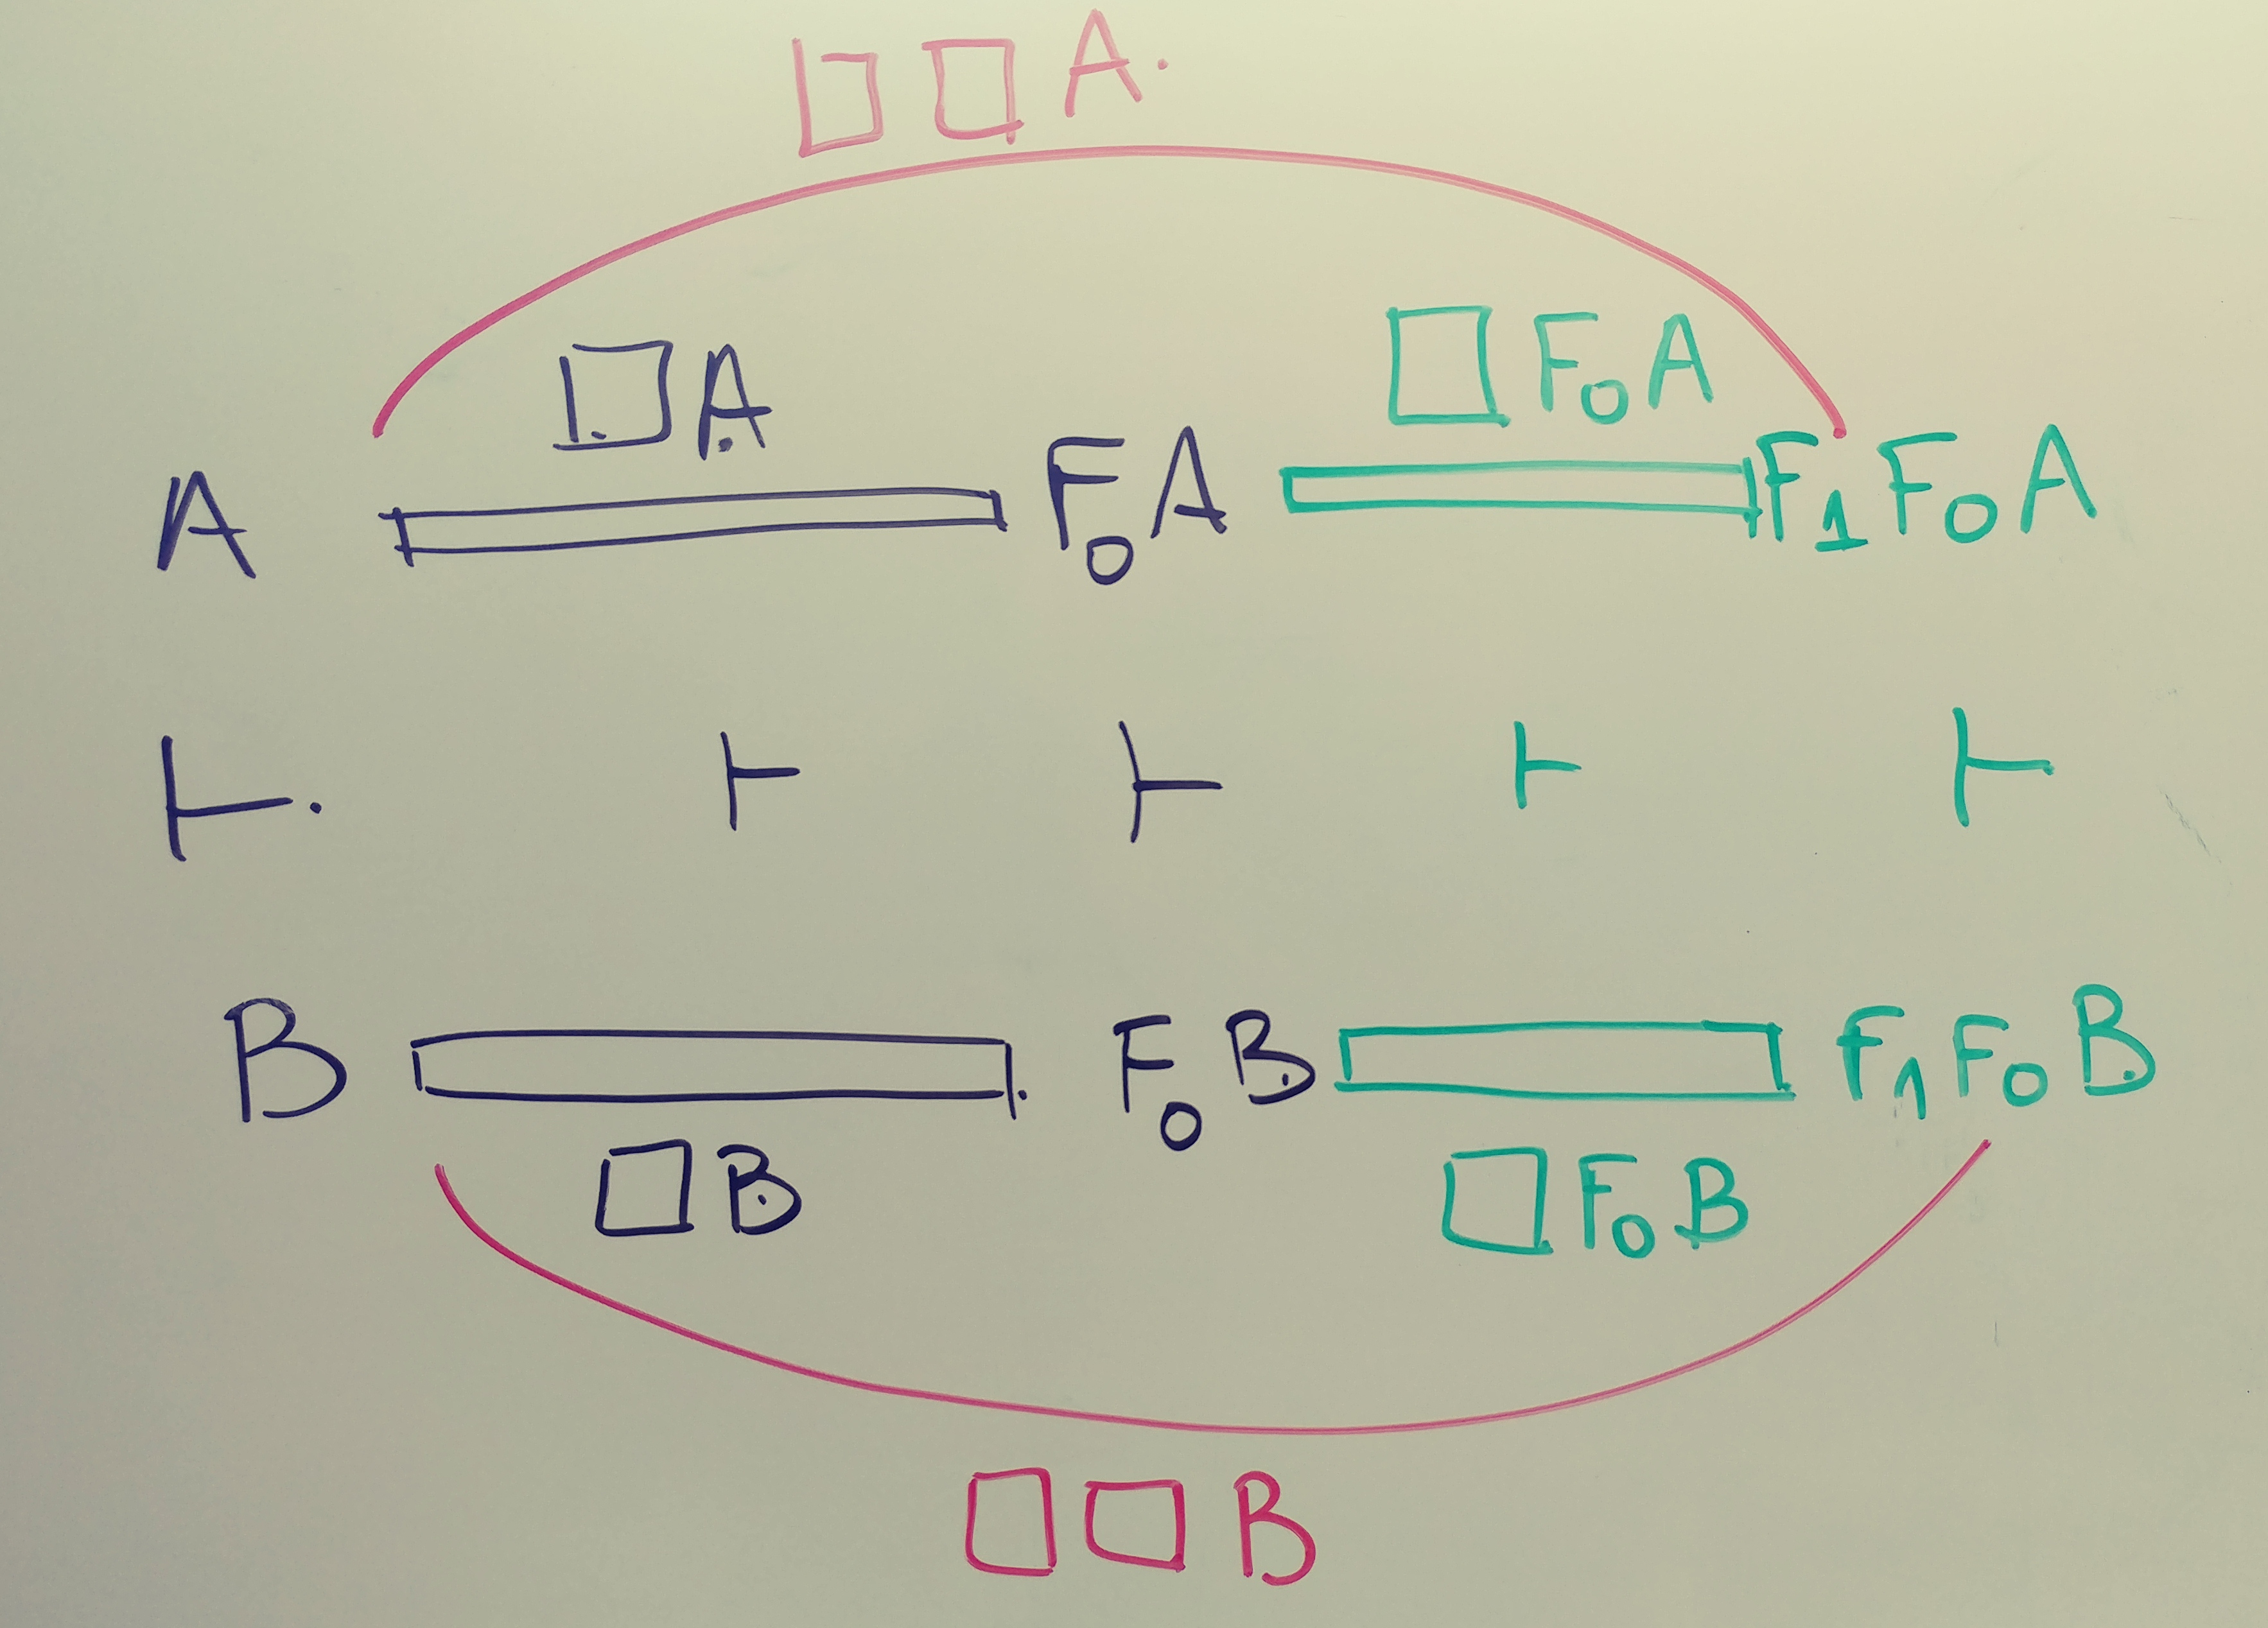
\includegraphics[scale=0.05]{pics/20171111_141413_Film1}
      \column{0.3\textwidth}
          Yes! Takes  a bit more syntax and using the bang operator of justification logic
    \end{columns}
      \end{frame}
  
    \begin{frame}{What about stronger modality?}
      A Galois connection is 
      a pair of order preserving functions $L:\mathcal{D}\rightarrow C$, $R:\mathcal{C}\rightarrow{D}$
      such that there is an isomorphism:
      $\forall d\in  D, c\in C. \  Ld\le c \longleftrightarrow d\le R c$
      
      Take the relation of classical and intuitionistic logic as a prototype:
      \begin{mathpar}
        \inferrule*[right=$\downarrow\uparrow$] {\llbracket\Gamma\rrbracket\vdash_{class}\phi}{\Gamma\vdash_I\neg\neg \phi}
    
      \end{mathpar}
    This is a typical case of a Galois connection (or an adjunction)\\
    To mimic such a notion in $Jcalc$ one should add another function symbol to 
    correspond to $R$ and add the rule:  
    \begin{mathpar}
        \inferrule*[right=$R$]{\llbracket\Gamma\rrbracket\vdash_J {\sf j}:\phi}
        {\Gamma\vdash {\sf eval\_return} \ \  {\sf j} :R\phi} 
    \end{mathpar}
    
    
    \end{frame}
    \begin{frame}
      This is enough to obtain a generalized notion of Factivity that is:
      \begin{mathpar}
          \inferrule*[right=$R$]{\Gamma\vdash M:\Box\phi}
          {\Gamma\vdash \sf {let} \ \_\_ \ \&\ s \ {\sf be\ } M \ \  {\sf in}\  {\sf eval\_return} (s):R\llbracket\phi\rrbracket} 
      \end{mathpar}  
     Ideas from the Artemov, Bonelli \textit{Intensional Lambda calculus} 
     could be utilized to add evaluation at the level of justifications
    \end{frame}  

    \begin{frame}{Concluding}
    \begin{itemize}
     \item[] Justification logic has rich  higher order features and reflection!
     \item[] I see this as a first part of a project for utilizing it 
      to provide foundations of \textit{typed programming language interaction} 
    \end{itemize}
  \end{frame}
    \begin{frame}
      Thank you!
    \end{frame}
  \end{document}
